\documentclass[]{article}
\usepackage{fullpage}
\usepackage[authoryear]{natbib}
\usepackage{setspace}
    \doublespacing
\usepackage{hyperref}
\hypersetup{
    colorlinks,
    citecolor=black,
    filecolor=black,
    linkcolor=cyan,
    urlcolor=cyan
}
\usepackage{amssymb,amsmath}
\usepackage{bm}
\usepackage{dcolumn}
\usepackage{booktabs}
\usepackage{url}
\usepackage{tikz}
\usepackage{todonotes}
\usepackage[utf8]{inputenc}
\usepackage{graphicx}
\usepackage{longtable}
\usepackage{todonotes}
\usepackage{lscape}
\usepackage{float}


\title{Fiscal Rule Stretching in Europe During Financial Market Stress and Crises}

\author{Christopher Gandrud \\ \emph{City University London} \\ \emph{Hertie School of Governance}\footnote{Please contact Christopher Gandrud
(\href{mailto:christopher.gandrud@city.ac.uk}{\nolinkurl{christopher.gandrud@city.ac.uk}}) or Mark Hallerberg (\href{mailto:hallerberg@hertie-school.org}{\nolinkurl{hallerberg@hertie-school.org}}).}
\and
Mark Hallerberg \\ \emph{Hertie School of Governance}}

\begin{document}

\maketitle

\begin{center}
    \textbf{Very Early Working Draft for\\ Texas A \& M University: Fiscal Policy in Europe Workshop (11 December 2015) \\
    Comments and suggestions very welcome.}
\end{center}

\begin{abstract}
    Elected governments have incentives to stretch accounting rules by classifying loss-making and/or indebted endeavors, such as public industries and pension schemes, as off of the public balance sheet. Doing so improves the appearance of the incumbent government to cost-conscious voters. We expect rule stretching to be especially prevalent during periods of financial market stress and crises given the typically high expense of responding to these events. In addition, types of policy options available to assist troubled financial institutions, such as bad banks and bank nationalizations, are often hard to classify as being inside or outside of the government sector, thus making it more likely that governments will tend to stretch how they are classified. To test these proposition, we examine revisions to government debt and deficit figures made by the European statistical agency--Eurostat. These revisions frequently occur because this politically independent agency re-classifies organizations as being within the government sector, when a national government had originally classified them as outside. We find that debt figures are more likely to be revised upwards for years close to national elections, especially when these are required non-endogenous elections. These effects are strengthened further by financial market stress. Our research underlines the importance of having a vigilant and politically independent government statistical agency during periods of financial market stress to ensure reliable government finance statistics.
\end{abstract}

\section{Introduction}

\section{Political budget cycles and fiscal gimmicks}

\cite{DeCastro2013} \cite{Alt2014}

\section{Cost-shifting during financial crises}

\cite{GandrudHallerberg2016}

\section{Hypotheses}

\begin{quote}
    $H_{1}$: Debt revisions will be greater for years closer to national government elections.
\end{quote}

\begin{quote}
    $H_{2}$: Debt revisions will be greater for years when there are required (non-endogenous) elections.
\end{quote}

\begin{quote}
    $H_{3}$: The effects predicted by $H_{1}$ and $H_{2}$ will be stronger when a country also has high credit provision stress.
\end{quote}

\section{Empirical tests}

\subsection{Eurostat revisions}

To test these hypotheses we gathered all of the revisions that Eurostat made to EU member debt and deficit figures from 2003 through 2013.\footnote{PDF files with the figures were downloaded from \url{http://ec.europa.eu/eurostat/news/news-releases}.} Eurostat publishes revisions bi-annually--typically once at the end of April and again again in late October. These revisions cover government finance statistics released within the previous four years. As such, the unit of analysis in the following regressions is biannual revision point for each fiscal year. For every year that government statistics are revised, there are up to seven revision points.\footnote{The first revisions occur October of the initial reporting year.}

We created a variable of \emph{cumulative revisions for debts and deficits} over these four year periods and used them as our dependent variables. For debt revisions, it ranged from -1.1 and 12.7 percent of GDP. For deficit revisions it ranged from -4.5 and 1.1 percent of GDP. It is important to note that all of these revisions were not due to revisions in the denominator, i.e. GDP. Eurostat reports these types of changes separately. As \cite{DeCastro2013} found for similar Eurostat data in shorter pre-financial crisis sample, there is a clear tendency for debt statistics to be revised upward and deficit statistics downward, indicating that policies are more expensive than initially reported.

\subsection{Right-hand variables}

To test whether governments are more likely to stretch the rules closer to elections, we use Gandrud's \citeyearpar{gandrudYrcurnt} \emph{years to election} variable. The election year is recorded as zero. Not only do we expect that governments are more likely to use rule stretching as elections approach, but that rule stretching should be more prevalent when governments are not able to choose the when the election occurs so as to present themselves in the best fiscal light to voters. As such, we also include a dummy variable that is one for \emph{required elections} (e.g. non-endogenous elections) and zero for all other years. The variable is from \cite{Brender2008}. It was updated and corrected by Hallerberg and Wehner. We expect that that revisions will be greater for years when there is a non-endogenous election.

To examine how responding to financial market stress may exacerbate governments' fiscal accounting rule stretching behavior, we included Gandrud and Hallerberg's \citeyearpar{finstress_paper} continuous ``FinStress'' measure of real-time perceptions of financial market stress. This measure is created by analyzing monthly content from Economist Intelligence Unit texts on banking and financial markets using a statistical method called kernel principal component analysis. Unlike previous post-hoc dichotomous measures of financial crisis \citep[e.g. measures compiled by][]{Laeven2012,ReinhartRog2010}, the authors argue this measure captures what we are most interested in when trying to understand policy choices: what stress policy-makers perceived and so responded to at the time. It also does not rely on ad hoc methods of determining when a crisis ended, but instead charts its perceived intensity over time. To make this measure comparable with our other variables, we found yearly averages. FinStress is able to vary between zero and one, with higher values indicating more perceived financial market stress. In the sample it varies between 0.12 and 0.76.

Because hypothesize that the effect of election timing on rule-stretching will increase at higher levels of financial market stress, we will focus on interacting FinStress with the election timing and non-endogenous elections variables.

As Eurostat has more time to examine member state government policies, e.g. how separate they are in practice from the government sector, we would expect on average that the cumulative revisions will grow over the course of the four year period during which they are revised. So we also include a variable counting the years since the original year that the revised figure is from on the right-hand side.


% Table created by stargazer v.5.2 by Marek Hlavac, Harvard University. E-mail: hlavac at fas.harvard.edu
% Date and time: Fri, Feb 12, 2016 - 14:39:59
\begin{table}[!htbp] \centering 
  \caption{Linear Regression Estimation of \textbf{Debt} Revisions} 
  \label{debt_results} 
\tiny 
\begin{tabular}{@{\extracolsep{5pt}}lccccccccccc} 
\\[-1.8ex]\hline 
\hline \\[-1.8ex] 
 & \multicolumn{11}{c}{\textit{Dependent variable:}} \\ 
\cline{2-12} 
\\[-1.8ex] & \multicolumn{11}{c}{Cumulative Debt Revisions} \\ 
\\[-1.8ex] & (1) & (2) & (3) & (4) & (5) & (6) & (7) & (8) & (9) & (10) & (11)\\ 
\hline \\[-1.8ex] 
 Cum. Revisions (lag) & 0.628$^{***}$ & 0.757$^{***}$ & 0.626$^{***}$ & 0.731$^{***}$ & 0.554$^{***}$ & 0.536$^{***}$ & 0.641$^{***}$ & 0.640$^{***}$ & 0.634$^{***}$ & 0.681$^{***}$ & 0.634$^{***}$ \\ 
  & (0.021) & (0.021) & (0.021) & (0.022) & (0.026) & (0.026) & (0.021) & (0.021) & (0.022) & (0.025) & (0.022) \\ 
  & & & & & & & & & & & \\ 
 Election Timing & 0.047$^{*}$ &  & $-$0.031 &  &  &  &  &  & $-$0.064 &  & $-$0.028 \\ 
  & (0.027) &  & (0.047) &  &  &  &  &  & (0.049) &  & (0.040) \\ 
  & & & & & & & & & & & \\ 
 Unscheduled Elect. &  & 0.229$^{*}$ &  & $-$0.560$^{**}$ &  &  &  &  &  & $-$0.576$^{**}$ &  \\ 
  &  & (0.132) &  & (0.235) &  &  &  &  &  & (0.248) &  \\ 
  & & & & & & & & & & & \\ 
 Scheduled Elect. &  & $-$0.001 &  & $-$0.057 &  &  &  &  &  & $-$0.157 &  \\ 
  &  & (0.073) &  & (0.128) &  &  &  &  &  & (0.150) &  \\ 
  & & & & & & & & & & & \\ 
 Financial Stress & 0.039 & 0.191 & $-$1.082$^{*}$ & $-$0.049 &  &  &  &  & $-$1.380$^{**}$ & $-$0.001 & 0.075 \\ 
  & (0.327) & (0.257) & (0.643) & (0.278) &  &  &  &  & (0.651) & (0.331) & (0.343) \\ 
  & & & & & & & & & & & \\ 
 Gen. Gov. Deficit &  &  &  &  & $-$0.004 & 0.010 &  &  &  &  &  \\ 
  &  &  &  &  & (0.011) & (0.011) &  &  &  &  &  \\ 
  & & & & & & & & & & & \\ 
 Cent. Gov. Debt &  &  &  &  & 0.004$^{*}$ & 0.004$^{*}$ &  &  &  &  &  \\ 
  &  &  &  &  & (0.002) & (0.002) &  &  &  &  &  \\ 
  & & & & & & & & & & & \\ 
 Euro Member &  &  &  &  & 0.233 & $-$0.479$^{*}$ & $-$0.006 & $-$0.066 &  &  &  \\ 
  &  &  &  &  & (0.183) & (0.272) & (0.194) & (0.201) &  &  &  \\ 
  & & & & & & & & & & & \\ 
 EDP &  &  &  &  &  &  & 0.163$^{**}$ & 0.041 & 0.175$^{**}$ & 0.083 & $-$0.145 \\ 
  &  &  &  &  &  &  & (0.080) & (0.131) & (0.082) & (0.081) & (0.155) \\ 
  & & & & & & & & & & & \\ 
 Elect. Timing*Fin. Stress &  &  & 0.506$^{**}$ &  &  &  &  &  & 0.658$^{***}$ &  &  \\ 
  &  &  & (0.250) &  &  &  &  &  & (0.252) &  &  \\ 
  & & & & & & & & & & & \\ 
 Unscheduled.Elect*Fin. Stress &  &  &  & 5.818$^{***}$ &  &  &  &  &  & 6.493$^{***}$ &  \\ 
  &  &  &  & (1.443) &  &  &  &  &  & (1.524) &  \\ 
  & & & & & & & & & & & \\ 
 Scheduled.Elect*Fin. Stress &  &  &  & 0.384 &  &  &  &  &  & 0.980 &  \\ 
  &  &  &  & (0.731) &  &  &  &  &  & (0.815) &  \\ 
  & & & & & & & & & & & \\ 
 Cent. Gov. Debt*Euro &  &  &  &  &  & 0.011$^{***}$ &  &  &  &  &  \\ 
  &  &  &  &  &  & (0.003) &  &  &  &  &  \\ 
  & & & & & & & & & & & \\ 
 EDP*Euro &  &  &  &  &  &  &  & 0.191 &  &  &  \\ 
  &  &  &  &  &  &  &  & (0.162) &  &  &  \\ 
  & & & & & & & & & & & \\ 
 Elect. Timing*EDP &  &  &  &  &  &  &  &  &  &  & 0.137$^{**}$ \\ 
  &  &  &  &  &  &  &  &  &  &  & (0.057) \\ 
  & & & & & & & & & & & \\ 
 Constant & 0.648$^{***}$ & 0.361$^{**}$ & 0.831$^{***}$ & 0.353$^{**}$ & 0.251 & 0.316 & 0.658$^{**}$ & 0.688$^{***}$ & 0.807$^{***}$ & 0.343$^{**}$ & 0.752$^{***}$ \\ 
  & (0.188) & (0.151) & (0.208) & (0.152) & (0.309) & (0.308) & (0.255) & (0.257) & (0.209) & (0.160) & (0.203) \\ 
  & & & & & & & & & & & \\ 
\hline \\[-1.8ex] 
Country FE? & Yes & Yes & Yes & Yes & Yes & Yes & Yes & Yes & Yes &  &  \\ 
Observations & 1,494 & 1,189 & 1,494 & 1,189 & 1,230 & 1,230 & 1,371 & 1,371 & 1,345 & 1,047 & 1,345 \\ 
R$^{2}$ & 0.546 & 0.655 & 0.547 & 0.660 & 0.397 & 0.403 & 0.546 & 0.546 & 0.548 & 0.636 & 0.548 \\ 
Adjusted R$^{2}$ & 0.537 & 0.646 & 0.538 & 0.651 & 0.384 & 0.390 & 0.536 & 0.536 & 0.538 & 0.625 & 0.537 \\ 
\hline 
\hline \\[-1.8ex] 
\textit{Note:}  & \multicolumn{11}{r}{$^{*}$p$<$0.1; $^{**}$p$<$0.05; $^{***}$p$<$0.01} \\ 
\end{tabular} 
\end{table} 



% Table created by stargazer v.5.2 by Marek Hlavac, Harvard University. E-mail: hlavac at fas.harvard.edu
% Date and time: Thu, Oct 27, 2016 - 13:37:08
\begin{table}[!htbp] \centering 
  \caption{Linear Regression Estimation of Deficit Revisions (Full Sample)} 
  \label{deficit_results} 
\tiny 
\begin{tabular}{@{\extracolsep{5pt}}lcccccccccc} 
\\[-1.8ex]\hline 
\hline \\[-1.8ex] 
 & \multicolumn{10}{c}{\textit{Dependent variable:}} \\ 
\cline{2-11} 
\\[-1.8ex] & \multicolumn{10}{c}{Cumulative Deficit Revisions} \\ 
\\[-1.8ex] & (1) & (2) & (3) & (4) & (5) & (6) & (7) & (8) & (9) & (10)\\ 
\hline \\[-1.8ex] 
 Revised Gen. Gov. Deficit & 0.053$^{***}$ & 0.042$^{*}$ & 0.042$^{*}$ & 0.048$^{***}$ & 0.049$^{***}$ & 0.049$^{***}$ & 0.038$^{**}$ & 0.050$^{***}$ & 0.033$^{**}$ & 0.098$^{**}$ \\ 
  & (0.013) & (0.020) & (0.020) & (0.013) & (0.013) & (0.013) & (0.013) & (0.014) & (0.011) & (0.030) \\ 
  & & & & & & & & & & \\ 
 Euro Member & $-$0.190 & $-$0.180 & $-$0.180 & $-$0.183 & $-$0.192 & $-$0.205 & $-$0.145 & $-$0.179 & $-$0.329 & $-$0.353 \\ 
  & (0.197) & (0.193) & (0.193) & (0.182) & (0.181) & (0.182) & (0.188) & (0.190) & (0.262) & (0.212) \\ 
  & & & & & & & & & & \\ 
 EDP & 0.340$^{**}$ &  &  &  &  &  &  &  &  & 0.346$^{**}$ \\ 
  & (0.104) &  &  &  &  &  &  &  &  & (0.112) \\ 
  & & & & & & & & & & \\ 
 Election Timing &  &  &  & $-$0.014 &  &  &  & $-$0.038 &  &  \\ 
  &  &  &  & (0.027) &  &  &  & (0.124) &  &  \\ 
  & & & & & & & & & & \\ 
 Unscheduled Elect. &  &  &  &  & $-$0.163 & 0.663 &  &  &  & 0.518 \\ 
  &  &  &  &  & (0.153) & (0.640) &  &  &  & (0.661) \\ 
  & & & & & & & & & & \\ 
 Scheduled Elect. &  &  &  &  & 0.115 & $-$0.197 &  &  &  & $-$0.349 \\ 
  &  &  &  &  & (0.090) & (0.369) &  &  &  & (0.427) \\ 
  & & & & & & & & & & \\ 
 Financial Stress &  &  &  & 0.008 & 0.009$^{*}$ & 0.009 &  & 0.007 &  & 0.005 \\ 
  &  &  &  & (0.004) & (0.004) & (0.005) &  & (0.008) &  & (0.006) \\ 
  & & & & & & & & & & \\ 
 Fiscal Transparency &  &  &  &  &  &  & $-$0.001 & $-$0.0003 &  &  \\ 
  &  &  &  &  &  &  & (0.003) & (0.003) &  &  \\ 
  & & & & & & & & & & \\ 
 GDP Growth &  &  &  &  &  &  & $-$0.008 & $-$0.003 &  & $-$0.004 \\ 
  &  &  &  &  &  &  & (0.010) & (0.010) &  & (0.012) \\ 
  & & & & & & & & & & \\ 
 Contracts &  &  &  &  &  &  &  &  & $-$0.669 &  \\ 
  &  &  &  &  &  &  &  &  & (1.999) &  \\ 
  & & & & & & & & & & \\ 
 Debt * Euro &  & $-$0.013 & $-$0.013 &  &  &  &  &  &  & $-$0.042 \\ 
  &  & (0.024) & (0.024) &  &  &  &  &  &  & (0.029) \\ 
  & & & & & & & & & & \\ 
 Elect. Timing * Fin. Stress &  &  &  &  &  & $-$0.017 &  &  &  & $-$0.016 \\ 
  &  &  &  &  &  & (0.013) &  &  &  & (0.013) \\ 
  & & & & & & & & & & \\ 
 Unscheduled Elect. * Fin. Stress &  &  &  &  &  & 0.007 &  &  &  & 0.011 \\ 
  &  &  &  &  &  & (0.008) &  &  &  & (0.009) \\ 
  & & & & & & & & & & \\ 
 Scheduled Elect. * Fin. Stress &  &  &  &  &  &  &  & 0.001 &  &  \\ 
  &  &  &  &  &  &  &  & (0.003) &  &  \\ 
  & & & & & & & & & & \\ 
 Constant & $-$0.322 & $-$0.303 & $-$0.303 & $-$0.654$^{*}$ & $-$0.696$^{*}$ & $-$0.704$^{*}$ & $-$0.265 & $-$0.551 & 0.464 & $-$0.428 \\ 
  & (0.267) & (0.259) & (0.259) & (0.314) & (0.310) & (0.324) & (0.273) & (0.457) & (1.839) & (0.381) \\ 
  & & & & & & & & & & \\ 
\hline \\[-1.8ex] 
Country FE? & Yes & Yes & Yes & Yes & Yes & Yes & Yes & Yes & Yes & Yes \\ 
Observations & 413 & 460 & 460 & 460 & 460 & 460 & 460 & 460 & 423 & 413 \\ 
R$^{2}$ & 0.286 & 0.267 & 0.267 & 0.274 & 0.279 & 0.283 & 0.268 & 0.274 & 0.265 & 0.306 \\ 
Adjusted R$^{2}$ & 0.232 & 0.216 & 0.216 & 0.221 & 0.225 & 0.226 & 0.215 & 0.216 & 0.215 & 0.240 \\ 
\hline 
\hline \\[-1.8ex] 
\textit{Note:}  & \multicolumn{10}{r}{$^{*}$p$<$0.05; $^{**}$p$<$0.01; $^{***}$p$<$0.001} \\ 
\end{tabular} 
\end{table} 


\subsection{Results}

Tables \ref{debt_results} and \ref{deficit_results} showing results from linear regressions with cumulative debt and deficit revisions, respectively, as the dependent variable. All models include country fixed effects.

We can see in Table \ref{debt_results} that election timing is estimated to have a negative effect on debt revisions in models where it is not interacted with FinStress. As the election timing variable is larger, i.e. the further away the next election, government debt figures tend to be revised less. Or stated another way, debt revisions are larger for years closer to elections. This finding is similar in direction and magnitude to what \cite{DeCastro2013} found with similar data over a shorter time-span. A new finding can be seen in model 2 of Table \ref{debt_results}. Debt revisions are larger in years where a government was required to hold an election compared to other years. We can see that, in line with our third hypothesis, these two effects increase for years that also have higher credit market stress as measured by the FinStress variable.

Figures \ref{me_finstress_elect} and \ref{me_finstress_required_elect} show marginal effects of the election variables at various levels of credit market stress. At high levels of FinStress, e.g. above 0.55, the marginal effect of being one more year removed from an election on debt revisions is

\begin{figure}
    \caption{Marginal Effect of Election Timing (years to election) at Various Levels of Financial Market Stress on Debt Revisions}
    \label{me_finstress_elect}

    \begin{center}
        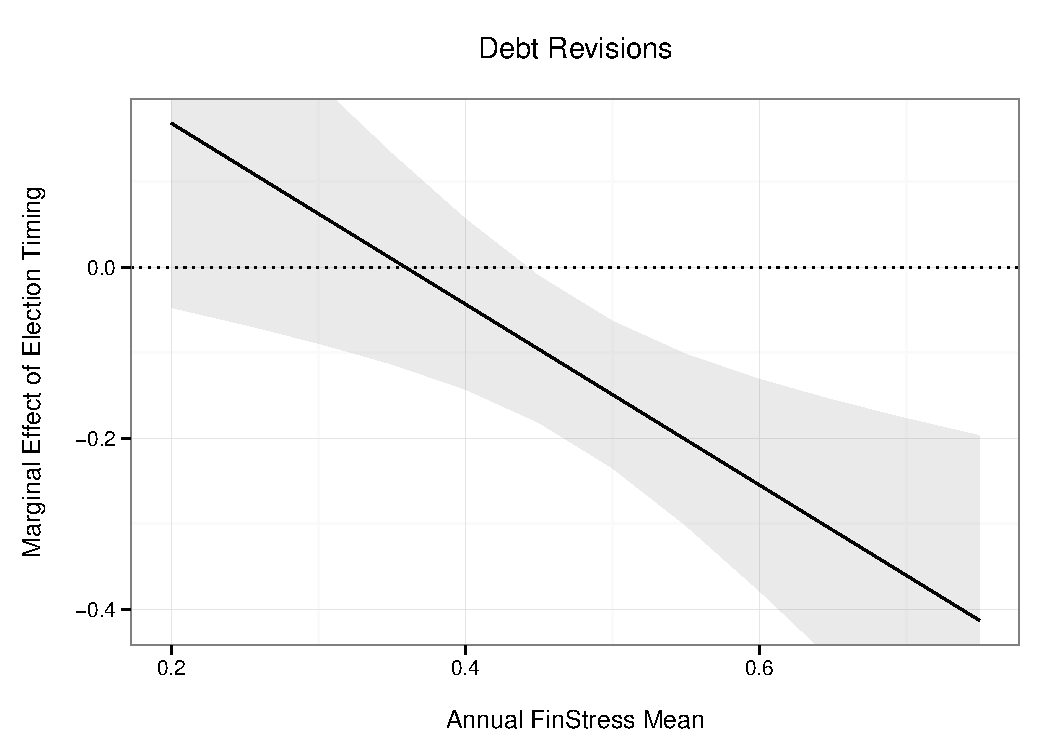
\includegraphics[scale=0.4]{figures/finstress_elect_me.pdf}
    \end{center}

	{\scriptsize{Shaded area represents 95\% confidence interval.}}

\end{figure}

\begin{figure}
    \caption{Marginal Effect of Non-Endogenous Elections at Various Levels of Financial Market Stress on Debt Revisions}
    \label{me_finstress_required_elect}

    \begin{center}
        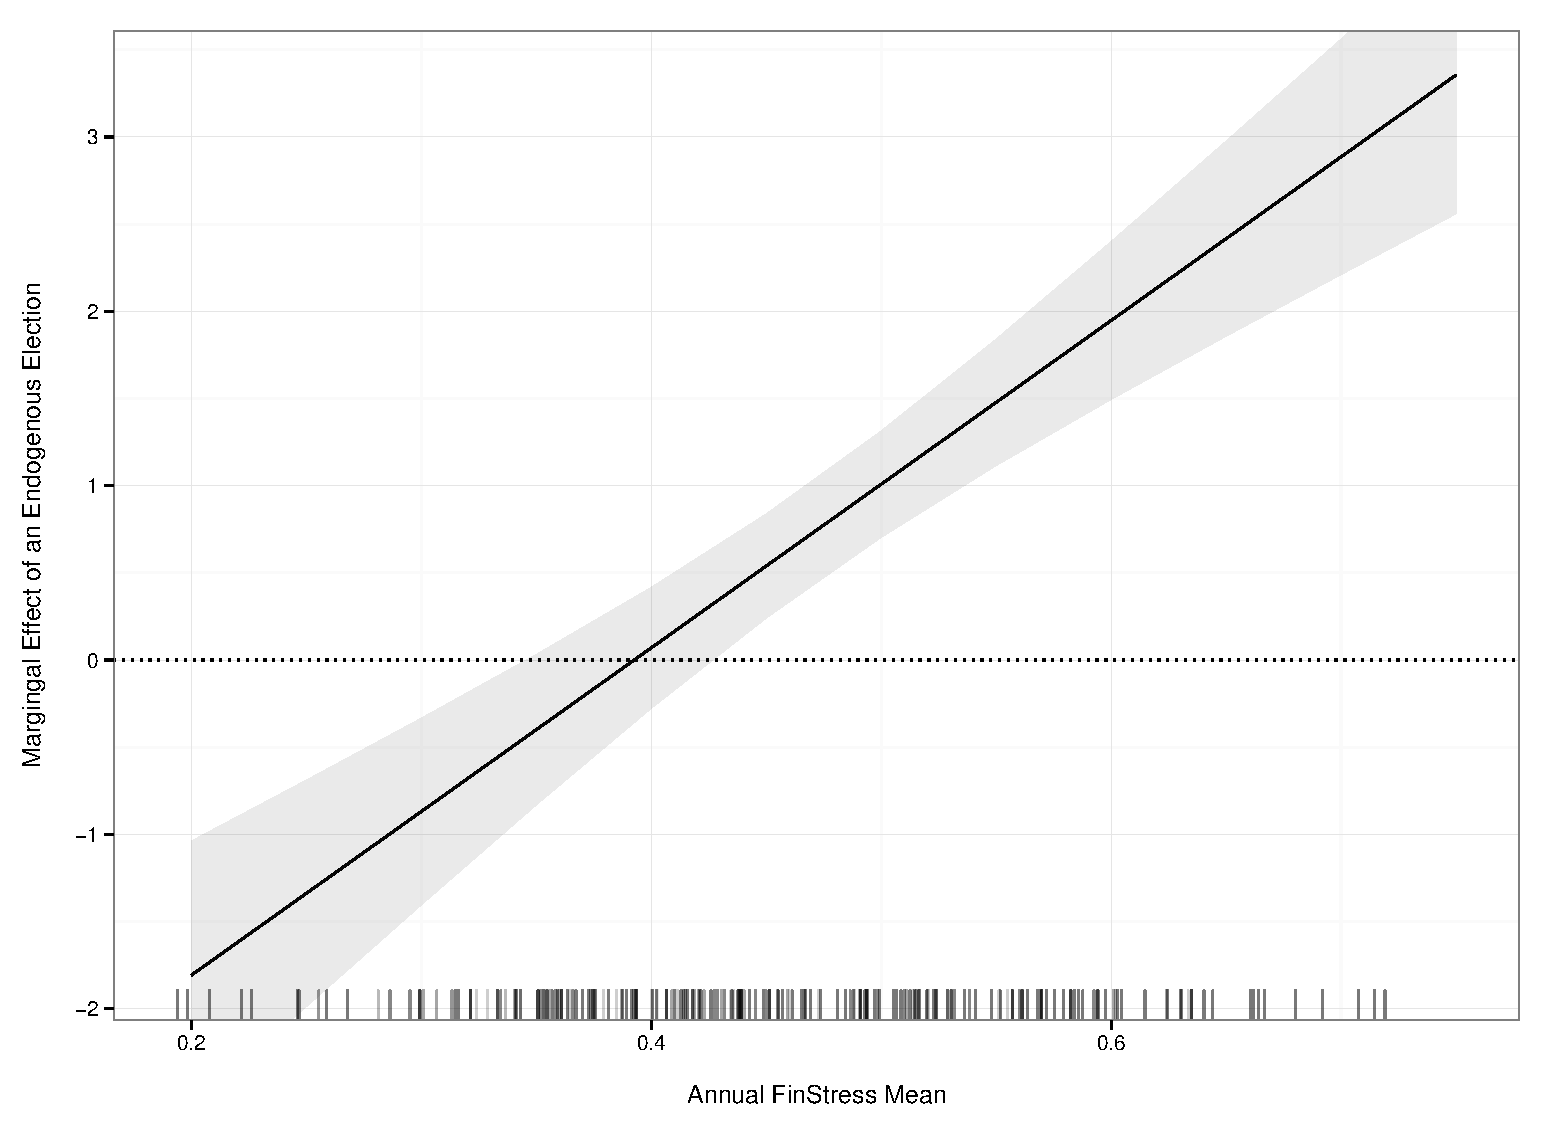
\includegraphics[scale=0.4]{figures/finstress_required_elect_me.pdf}
    \end{center}

	{\scriptsize{Shaded area represents 95\% confidence interval.}}

\end{figure}

\begin{figure}
	\caption{Predicted Debt Revisions in Three Years After Publication for Years with Non-Endogenous Elections vs. All Other Years}
    \label{country_predict_debt_required}
    \begin{center}
    	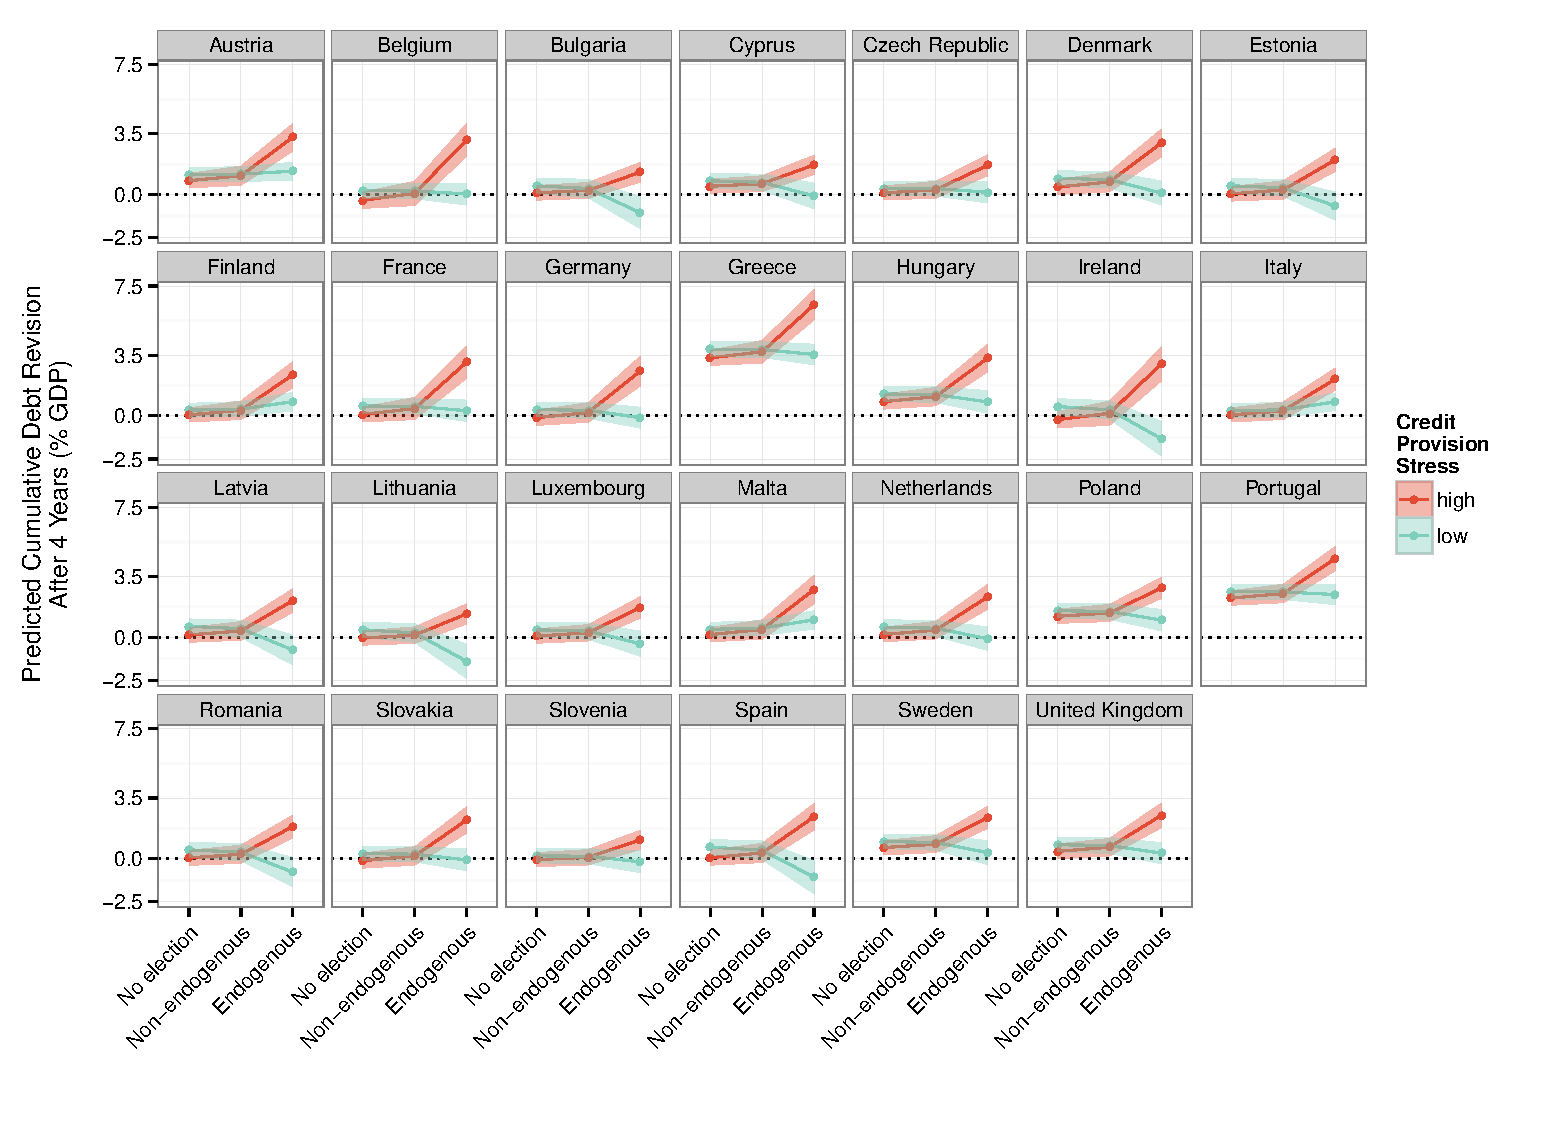
\includegraphics[scale=0.7]{figures/country_predict_required.pdf}
    \end{center}

	{\scriptsize{High and Low stress values refer to country minimum and maximum FinStress scores in the sample.\\
    Croatia excluded due to a small number of revision years.\\
    Shaded areas show 95\% confidence intervals.
}}

\end{figure}


\section{Conclusion}


\clearpage

\bibliographystyle{apsr}
\bibliography{main.bib}

\end{document}
